\documentclass[12pt, letterpaper]{article}
\usepackage{amsthm}
\usepackage{enumitem}
\usepackage{amsmath}
\usepackage{amssymb, mathtools}
\usepackage{graphicx}
\graphicspath{ {./images/} }
\title{CS 381 Homework 1}
\author{Ivan Chan \textit{933821369}}
\begin{document}
  
\textbf{CS 381 Homework 1}

Goal: Research and Explore a new programming language

\begin{enumerate}
  \item Select a programming language you have not used (NOT Haskell or Prolog). Give a brief history of this
  language. Who developed the language? When? Where?
    
  The programming language Python was created by Guido van Rossum with Python's first release on February 20, 1991.

  \item Give a description of the language. What is its paradigm(s)? How is it categorized? Describe some of
  the features of the language. What is typing method/discipline?
  
  Python is a high-level language and has an emphasis on code readability. It consists of garbage collection and is dynamically typed.
  Moreover, it can support functional, structured, and object oriented programming. Python is one of the most popular languages and this can be seen by its expansive library

  \item Is the language compiled or interpreted? On what platforms is the language available? Is the
  language standardized? Are there different implementations?

  The language is available on all platforms such as Linux, Windows, and macOS. Python is an interpreted language as its source code is converted into bytecode and executed.
  Its code is not required to be linked and compiled unlike languages such as C or C++.
  Standardized languages consists of a formal, approved standard written by an organization. Python is an open source language and thus not formally standardized.
  Finally, the known implementations of Python are IronPython, Jython, and PyPY.

  \item  Give examples of at least two control structures in the language (ie. for-loop or if-statement). Explain.
  
  \begin{enumerate}
    \item if-statement\\
    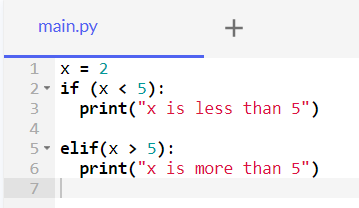
\includegraphics[scale = 0.8]{control1.PNG}\\
    In this case, the program dynamically creates a variable of x setting it equal to 2.\\
    It is ran through the control if statement to assess whether the variable is less than 5.\\
    If it is, print that x is less than 5.\\
    Else, we assess in an else if statement whether the variable x is less than 5\\
    If it is, print that x is more than 5.
    \item for-loop\\
    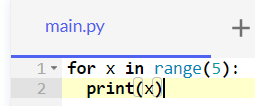
\includegraphics[scale = 0.8]{control2.PNG}\\
    For a variable that is within the range of x,\\
    Print the iterating numerical values that x becomes\\
    In this case, it will iterate through 0, 1, 2, 3, 4\\
    As it is a range of 5 includes 0 to 4.
  \end{enumerate}
  
  \item  To complete questions 6- 8 you will need to find an online\\ complier/interpreter to run code in your
  language, \\for example https://onecompiler.com/. \\Alternatively you can install the software or use the
  school’s server. What will you be using? 

  \underline{Note:}  You can use code you find online to answer questions 6-8 just include this information in the
  reference list for question 9.

  \item Write a “Hello World” program written in the language. Describe how it works. Provide a screenshot
  of the execution of the program.
    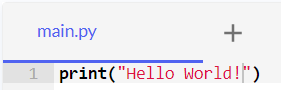
\includegraphics[scale = 0.8]{hello.PNG}\\
    Python takes any number of parameters given in the print() funciton and prints them all out in a single line\\
    The items are converted into text and a newline character is placed at the end of the string.

  \item Write a program to compute the first n Fibonacci numbers where the user is prompted for n (if
  possible). Describe how the code works. Is the program iterative or recursive? Provide a screenshot of
  the execution of the program.

    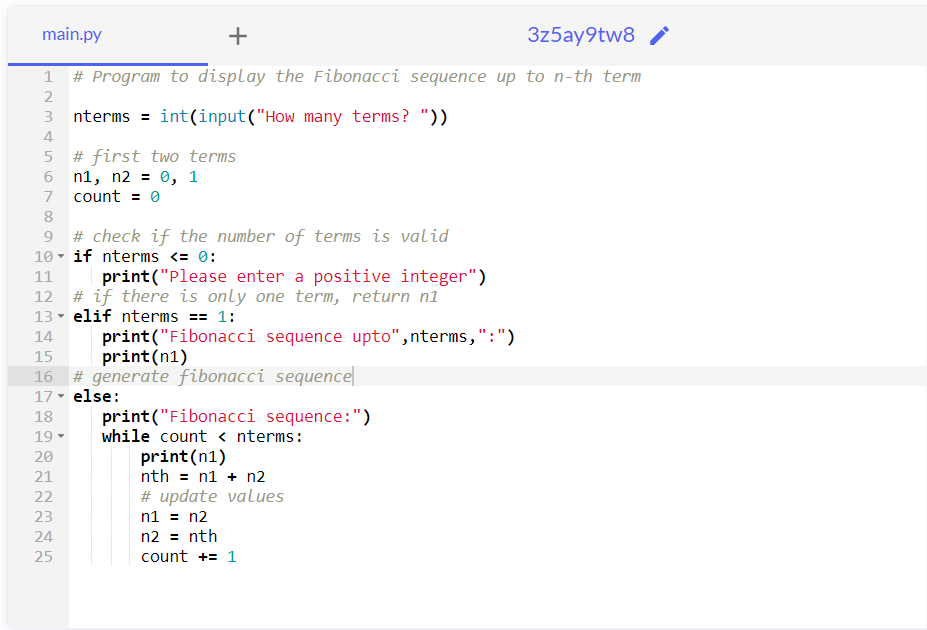
\includegraphics[scale = 0.5]{fibcode.PNG}
    \begin{enumerate}
      \item Variable n terms is casted as an int for user input for number of terms
      \item The first two terms are defined and set equal to 0 and 1
      \item A counter is defined and set to 0
      \item if the number of terms are less than or equal to 0
      \begin{enumerate}
        \item The user inputted a negative integer and reprompt
      \end{enumerate}
      \item Else if if the numebr of terms is just 1
      \begin{enumerate}
        \item Print the first fibonacci sequence
      \end{enumerate}
    \item else
    \begin{enumerate}
      \item while the counter is less than the number of terms inputted by user
      \begin{enumerate}
        \item print the first value
        \item have a new variable be the sum of the first and second values of the sequence
        \item set the first value as the second
        \item set the second as the sum
        \item increase the counter
      \end{enumerate}
    \end{enumerate}
    \end{enumerate}
    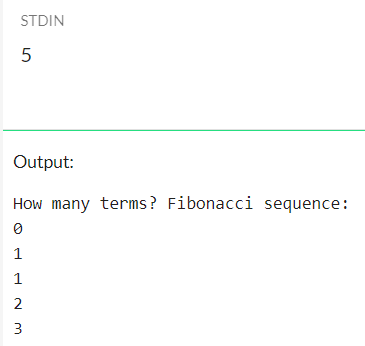
\includegraphics[scale = 0.5]{fiboutput.PNG}\\
    The program shows to be an iterative implementation of the fibonacci sequence.

  \item  Write a program to sort a list of integers. You can use any sorting algorithm, but do not use library
  functions. Describe how the code works. Provide a screenshot of the execution of the program.
  
  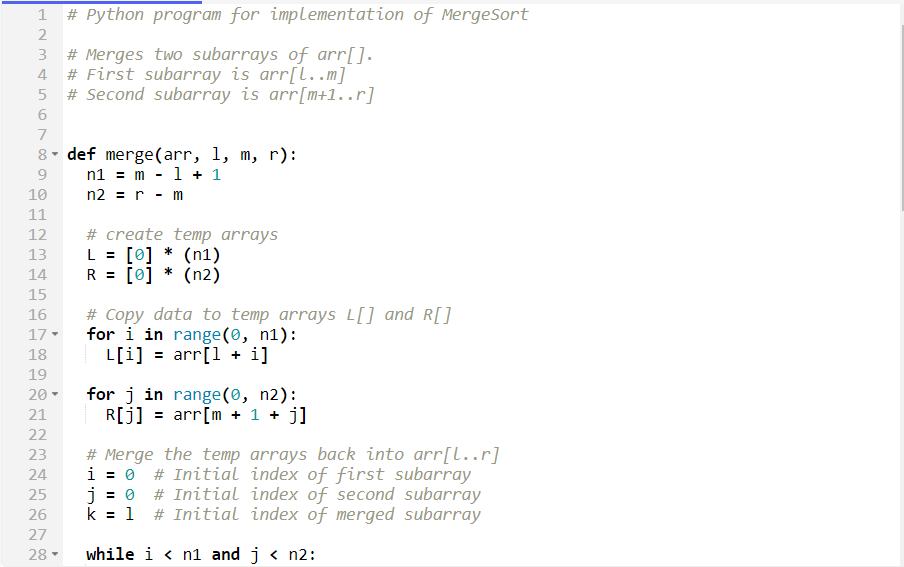
\includegraphics[scale = 0.5]{sort1.PNG}\\
  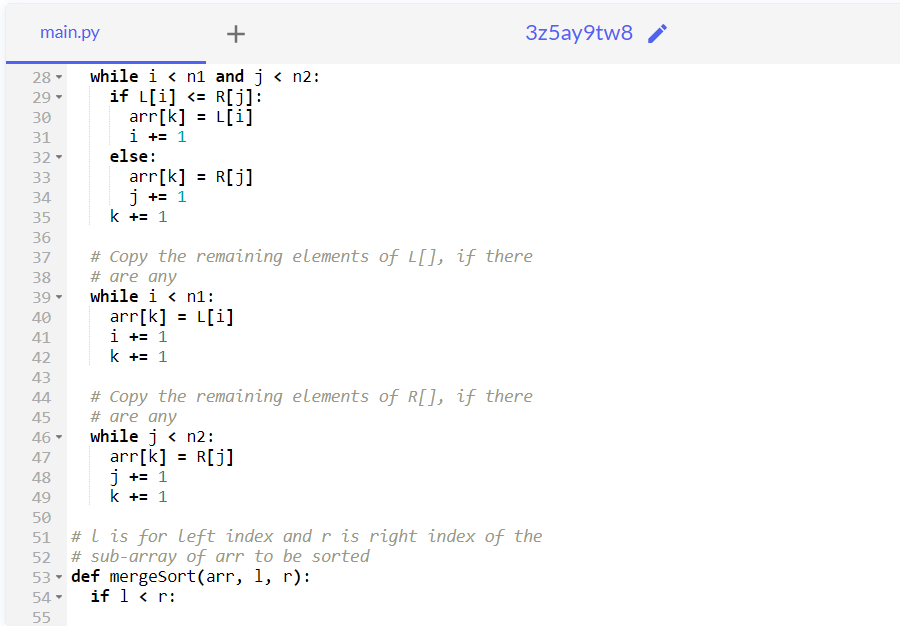
\includegraphics[scale = 0.5]{sort2.PNG}\\
  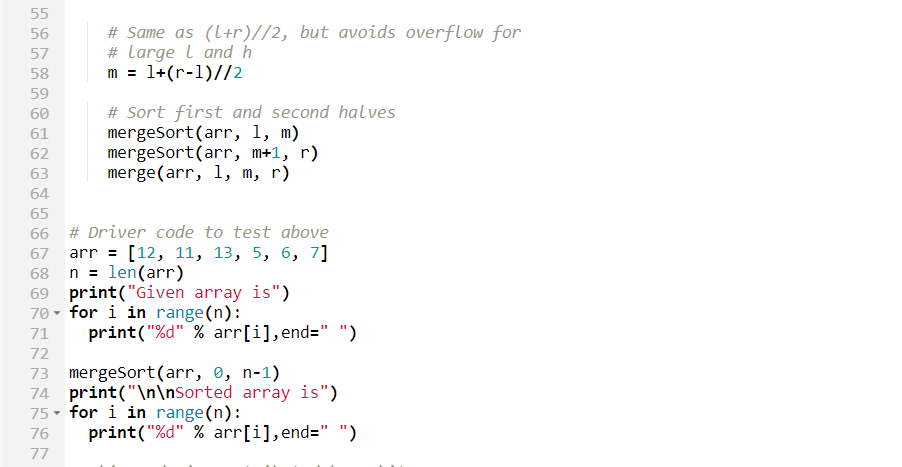
\includegraphics[scale = 0.5]{sort3.PNG}

  The implementation uses a merge sort algorithm in Python. Merge sort is a divide and conquer algorithm in which case\\
  The array that is to be sorted is havled into two different sub-arrays.\\
  This process is repeated for those two halves until all sub-arrays are sorted.\\
  Ultimately, all sub-arrays are merged.
  This algorithm has a time complexity of $O(n*\log(n))$
  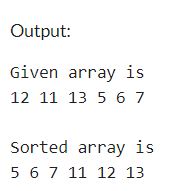
\includegraphics[scale = 0.5]{sortoutput.PNG}

  \item List at least three references you used for this assignment. Include any sites that you used to obtain
  code
  
  Python history:\\
  https://pythoninstitute.org\\

  Python control statements:\\
  https://www.w3schools.com/python/python_for_loops.asp\\

  Python fibonacci sequence code:\\
  https://www.programiz.com/python-programming/examples/fibonacci-sequence\\

  Python merge sort algorithm:\\
  https://www.geeksforgeeks.org/python-program-for-merge-sort/



  \item  Would you like to learn more about this language? Would anticipate using this language in the
  future? Explain

    Yes, python is a popular language and I would recommend it to people who would like to get their toes into coding or computer science.
    It is a high-level language and it is easy to understand with its simply readability.
\end{enumerate}
    

\end{document}
